\documentclass[../../thesis.tex]{subfiles}

\begin{document}

\TODO{Introduce the section, what we think and the philosophy of presenting material in such a way.}



\section{Neural Network}

\textit{Feedforward neural network}, \textit{artificial neural network}, \textit{multilayer perceptron} or simply \textit{neural network} is a fundemental model in machine learning, and more specifically in \textit{deep learning}. They are loosely inspired by biological neural systems.

\TODO{History}
\TODO{Sneak in something about universal approximation theorem}

A very general model


An artificial neural network is an $n$-fold iteration of affine transformations followed by some non-linear \textit{activation function}.

An artificial neural network is a linear combination of non-linear functions. It is parameterized by a set of \textit{weight} matrices $W_i$ and \textit{bias} vectors $\beta_i$, together with a specified non-linear \textit{activation function} $\sigma$. One can regard a ANN as a weighted directed acyclic graph, whose nodes are organized in layers and where the weights at a given layer is given by the weight matrices.


where the evaluation of $\sigma$ is pointwise. The calculation of $y$ using the network parameters is referred to as a \textit{feedforward operation}.

We stress that $\sigma$ is non-linear, as the composition of linear functions is linear, choosing a linear $\sigma$ would result in a linear $f_\theta$, which makes the network model equivalent to linear regression. Common non-linear activation functions include the sigmoid function, defined as $\sigma(x) = \frac{1}{1+e^{-x}}$, and the Rectified Linear Unit (ReLU), defined as $\sigma(x) = \text{max}(0, x)$. 

\begin{enumerate}
    \item nodes
    \item weights and biases (parameters)
    \item activation function
    \item input, hidden and output layers
\end{enumerate}

\section{Convolutional Neural Network}



\section{Residual Neural Network}


\section{Representation Learning}

\TODO{Sneak in something about Gödel and Turing in terms of representation}

\subsection*{What is representation learning?}
Representation learning is a term not too easily defined, one reason being the abstraction level. It relates closely to \textit{representation} of information, and representation of information can be many things. Lets begin by walking through a familiar and illustrative example. Consider the base $10$ integer $4$, or your favourite number. The number can equivalently (in terms of information content) be expressed, that is represented, in any other base. The particular base we choose depends on our intention with the number. If we want to work with digital electronics, a binary representation ($10$) is very useful, as transistors has two states. When humans do arithmetic, base $10$ representations of the integers are very natural, as we have $10$ fingers. A particular representation of information can make a task easier or harder.
\\
The information content is unchanged by a change of representation between $4$ in base $10$, $10$ when written in base $2$ or \RN{4} when written in roman numerals. What is changed is the challenges or easiness or difficulty of certain information processing tasks. Representation learning is then the process of learning a certain representation of information. 

\subsection*{What is a good representation?}

For any representations extracted of a non-invertible function, a downstream task can always be designed (in principle) to based on the lost information, hence achieve arbitrarily bad performance. The concept of universally good representations is therefore ill-defined. There is no free lunch in representation learning either. One must specify a set of predefined downstream tasks, and evaluate according to those. The goodness of a representation is determined by how easy it makes a subsequent task.

\subsection*{Why do we care about representation learning?}

Representation learning is particularly interesting because it provides one way to perform unsupervised and semi-supervised learning. It promises to unlock deep learning for unlabeled datasets. Furthermore it is known that the performance of machine learning methods is heavily dependent on the choice of data representations. Therefore much of actual efforts in deploying machine learning algorithms revolves around constructing good data pipelines and data transformations that results in representations suited for the ML algorithm. Being able to automate such processes, i.e automatic feature engineering, would solve massive problems and ease the use of ML considerably.

\section{Transformers}


Wiki: A deep learning architecture based on the multi-headed attention mechanism proposed in the 2017 paper "Attention is all you need".

\subsection{The attention mechanism}

\begin{figure}[h]
    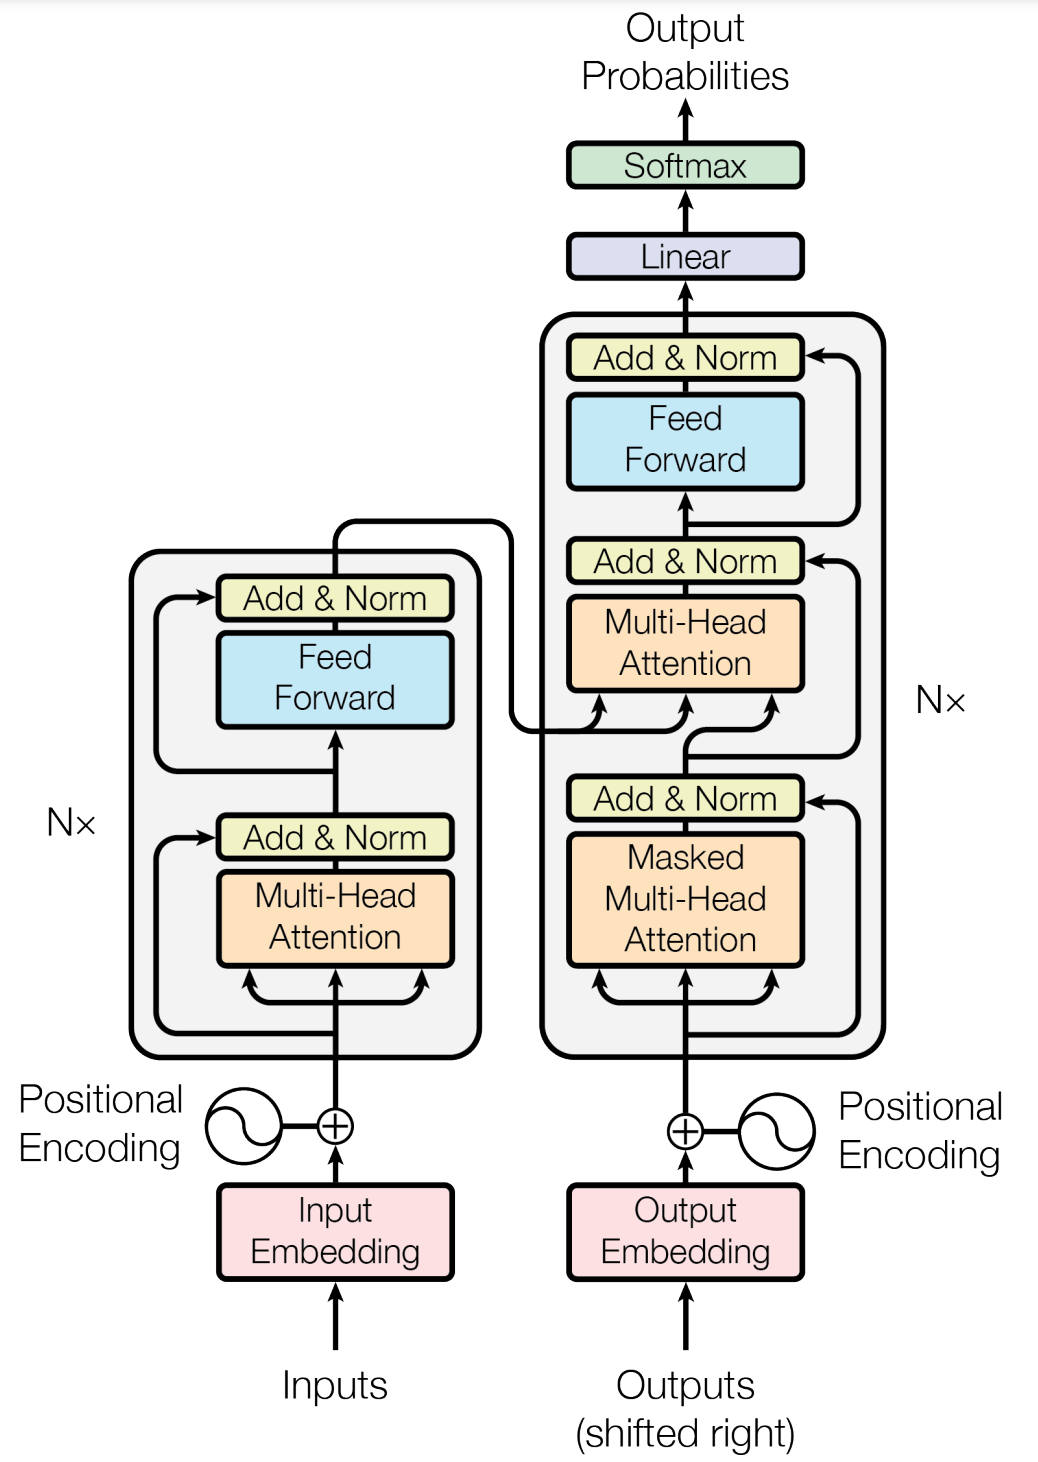
\includegraphics[scale=0.5]{Transformer_architecture}
    \centering    
\end{figure}



\subsection{Architecture}

Tokenizer

Positional encoding


Transformer layer (encoder/decoder)



\section{VQVAE}

\subsection{Variational Autoencoder}


- Encoder network which parameterizes the approximate posterior distribution $q(z|x$) of latent variables $z$ given the data $x$.
- Prior $p(z)$
- Decoder with distribution $p(x|z)$. 
- Note that we get the joint distribution $p(z)p(x|z) = p(x,z)$

ELBO and why

ELBO is a lower bound for the log likelihood of the data.

Maximizing ELBO w.r.t $\phi, \theta$  will concurrently (simultaneously)
- Approximately maximize the marginal likelihood $p_\theta(x)$ 
	- Generative model gets better
- Minimize the KL-divergence of the approximate posterior to true posterior. 
	- $q(z|x)$ becomes better

\subsection{Vector Quantized Variational Autoencoder}


\section{Self-supervised Learning}
\subsection{Siamese networks}
\subsection{Barlow Twins}

\section{MaskGIT}



\end{document}